% !TeX encoding = windows-1250
\chapter{Odnosni parametri kvalitete}

%Parametar se definira tako i tako

Parametar - varijabla o kojoj ovisi odre�eni logi�ki izraz, matemati�ka formula ili funkcija, a koju promatramo kao dodatnu ovisnost u izrazu koji se definira kao da je ta vrijednost �vrsta.

\section{Zajedni�ki, objektivni kriteriji usporedbe}

-Isti grad\\
-Isto doba godine\\
-Isto vremensko razdoblje
-Week day, work day

Kod generiranja matrica treba definirati ho�e li se putovanja koja se prote�u kroz vi�e perioda dodijeliti vremenskom periodu u kojem zapo�inju ili u kojem zavr�avaju. Iako ponekad nije specificirano, \cite{Bera:2011.} \cite{Filic:2016.} sva putovanja dodjeljuju intervalu u kojem je putovanje zapo�eto. 
cite{Netko:nekad} Ne zanemaruje one zapise iz kojih nije jasno vidljiv po�etak putovanja ve� takva putovanja dodjeljuje na osnovu vjerojatnosti da je zapo�elo u odre�enom periodu.

-Ima li matrica diagonalu? - kada se preslikava bs �elije na drugi oblik, 
nastaju putovanja unutar novih �elija (koje su ve�e od bs �elija) \cite{Graells-Garrido:2016.}  

\section{Komparacijski indikatori}

\subsection{Prostorna razlu�ivost (Rezolucija)}

Prema hrvatskoj enciklopediji definicija razlu�ivosti (rezolucije) glasi: mjera za razaznavanje sitnih pojedinosti na nekom prikazu (npr. televizijskoj slici). U ra�unalstvu se odnosi na fino�u rasterske slike iskazanu ukupnim brojem slikovnih elemenata (relativna razlu�ivost) ili brojem slikovnih elemenata po in�u (stvarna razlu�ivost).
to�nost polo�aja

\begin{figure}[!htbp]
	\begin{center}
		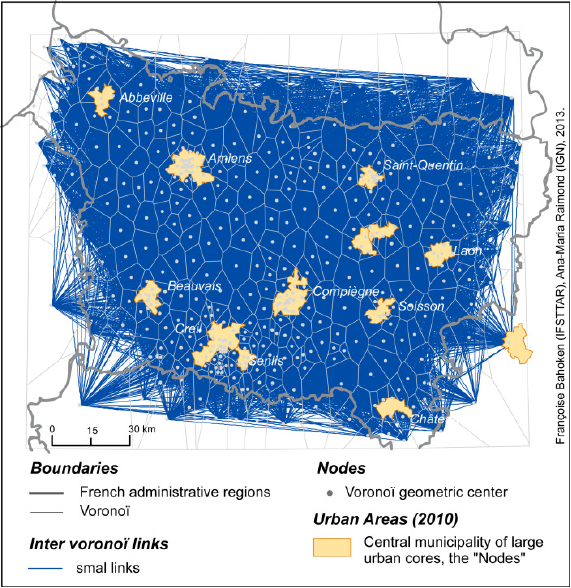
\includegraphics[width=10cm,keepaspectratio=true]{spaghetti_effect}
		\caption{\textit{Spaghetti-effect} - problem koji se mo�e javiti kod grafi�kog prikaza tokova matrice prikaz matrica visoke prostorne rezolucije \cite{Bahoken:2013.}}
		\label{fig:Revisiting}
	\end{center}
\end{figure}


\subsection{Vremenska razli�ivost}

Departure/Arrival time

\subsubsection{Dani u tjednu - radni dani/petak/vikend}

\subsubsection{Sezonske razlike}


\subsection{�irina toka}

Ukupan broj odlazaka/dolazaka po vremenskom okviru za cijelu matricu.\\
-Obuhva�a pje�a�ki promet


%\subsection{Geometrija prostorne podjele}
%(ne)uniformna podjela ...
%Interpolacija - ima li smisla 2 razli�ite podjele?!

\subsection{Definicija putovanja}

\subsubsection{Infrastruktura}
Obuhva�a pje�a�ki promet
%\subsubsection{Sredstvo kretanja}

\subsection{Gusto�a informacija - kontekst}


\section{Me�uovisnost parametara}
Ukoliko je rezlucija mala (velike �elije) nema potrebe za preciznim definiranjem kraja

\begin{comment}
2 modela
PoV (Predicted vs Observed)

Robusnost matrice ->una�anje �uma

\cite{Zhao:2017.} kad spominje TAD
\end{comment}

